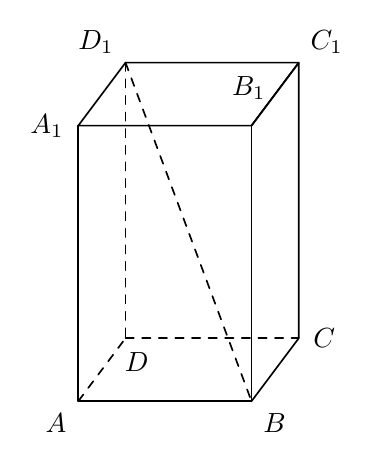
\begin{tikzpicture}[line width=.6pt, line join=round, line cap=round]
% 正四棱柱 ABCD-A1B1C1D1
\coordinate (A) at (0,0);
\coordinate (B) at (2.2,0);
\coordinate (C) at (2.8,0.8);
\coordinate (D) at (0.6,0.8);
\coordinate (A1) at (0,3.5);
\coordinate (B1) at (2.2,3.5);
\coordinate (C1) at (2.8,4.3);
\coordinate (D1) at (0.6,4.3);
% front face solid
\draw (A) -- (B) -- (B1) -- (A1) -- cycle;
% top face solid
\draw (A1) -- (B1) -- (C1) -- (D1) -- cycle;
% right face solid
\draw (B1) -- (B);
\draw (B) -- (C) -- (C1) -- (B1);
% hidden dashed
\draw[dashed] (D1) -- (D);
\draw[dashed] (D) -- (C);
\draw[dashed] (A) -- (D);
\draw[dashed] (D1) -- (B);
% labels with clearance
\node[font=\normalsize, inner sep=1pt, below left, xshift=-3pt, yshift=-3pt] at (A) {$A$};
\node[font=\normalsize, inner sep=1pt, below right, xshift=3pt, yshift=-3pt] at (B) {$B$};
\node[font=\normalsize, inner sep=1pt, right, xshift=4pt] at (C) {$C$};
\node[font=\normalsize, inner sep=1pt, below, xshift=4pt, yshift=-4pt] at (D) {$D$};
\node[font=\normalsize, inner sep=1pt, left, xshift=-4pt] at (A1) {$A_{1}$};
\node[font=\normalsize, inner sep=1pt, above, xshift=-1pt, yshift=8pt] at (B1) {$B_{1}$};
\node[font=\normalsize, inner sep=1pt, above right, xshift=3pt, yshift=2pt] at (C1) {$C_{1}$};
\node[font=\normalsize, inner sep=1pt, above left, xshift=-3pt, yshift=2pt] at (D1) {$D_{1}$};
\end{tikzpicture}
